\documentclass[12pt]{article}
\usepackage{graphicx}
\usepackage[none]{hyphenat}
\usepackage{graphicx}
\usepackage{listings}
\usepackage[english]{babel}
\usepackage{graphicx}
\usepackage{caption} 
\usepackage{booktabs}
\usepackage{array}
\usepackage{amssymb} % for \because
\usepackage{amsmath}   % for having text in math mode
\usepackage{extarrows} % for Row operations arrows
\usepackage{listings}
\lstset{
  frame=single,
  breaklines=true
}
\usepackage{hyperref}
  
%Following 2 lines were added to remove the blank page at the beginning
\usepackage{atbegshi}% http://ctan.org/pkg/atbegshi
\AtBeginDocument{\AtBeginShipoutNext{\AtBeginShipoutDiscard}}
\usepackage{gensymb}


%New macro definitions
\newcommand{\mydet}[1]{\ensuremath{\begin{vmatrix}#1\end{vmatrix}}}
\providecommand{\brak}[1]{\ensuremath{\left(#1\right)}}
\providecommand{\sbrak}[1]{\ensuremath{{}\left[#1\right]}}
\providecommand{\norm}[1]{\left\lVert#1\right\rVert}
\providecommand{\abs}[1]{\left\vert#1\right\vert}
\newcommand{\solution}{\noindent \textbf{Solution: }}
\newcommand{\myvec}[1]{\ensuremath{\begin{pmatrix}#1\end{pmatrix}}}
\let\vec\mathbf


\begin{document}

\begin{center}
	\title{\textbf{Normal to a Parabola}}
\date{\vspace{-5ex}} %Not to print date automatically
\maketitle
\end{center}
\setcounter{page}{1}

\section{12$^{th}$ Maths - Chapter 6}
This is Problem-22 from Exercise 6.6 
\begin{enumerate}
\item Find the equation of the normal at the point $(1,1)$ on the curve $2y + x^2 = 3$. 

\solution 
The given equation can be written as  
\begin{align}
	\label{eq:parabolaEq2}
	g\brak{\vec{x}} = \vec{x}^T\vec{V}\vec{x} + 2\vec{u}^T\vec{x} + f = 0 
\end{align}
where
\begin{align}
	\label{eq:eqV}
	\vec{V} &= \myvec{ 1 & 0 \\ 0 & 0} \\
	\label{eq:eqU}
	\vec{u} &= \myvec{0 \\ 1} \\
	\label{eq:eqF}
	f &= -3 
\end{align}
The equation of normal to the parabola , at a given point $\vec{q}$ is given by
\begin{align}
	\label{eq:EqNormal}
	\brak{\vec{V}\vec{q}+\vec{u}}^\top \vec{R}\brak{\vec{x}-\vec{q}}&= 0
\end{align}
where $\vec{R}$ is rotation matrix given by
\begin{align}
	\myvec{0 & -1 \\
	       1 & 0}
\end{align}
Given
\begin{align}
	\vec{q} &= \myvec{1 \\ 1} \\
\end{align}
Substituting all the values in \eqref{eq:EqNormal} 
\begin{align}
	&	\eqref{eq:EqNormal} \implies \brak{\myvec{1 & 0 \\ 0 &0}\myvec{1 \\ 1}+\myvec{0 \\ 1}}^\top \myvec{0 & -1 \\ 1 & 0}\brak{\vec{x}-\myvec{1 \\1}}= 0 \\
	&\implies \myvec{1 & 1 }\myvec{0 & -1 \\ 1 & 0}\brak{\vec{x}-\myvec{1 \\1}}= 0 \\
	&\implies \myvec{1 & -1 }\brak{\vec{x}-\myvec{1 \\1}}= 0 \\
	&\implies \myvec{1 & -1 }{\vec{x}} = 0 
\end{align}
The relevant figure is shown in \ref{fig:Fig1}
\begin{figure}[!h]
	\begin{center}
		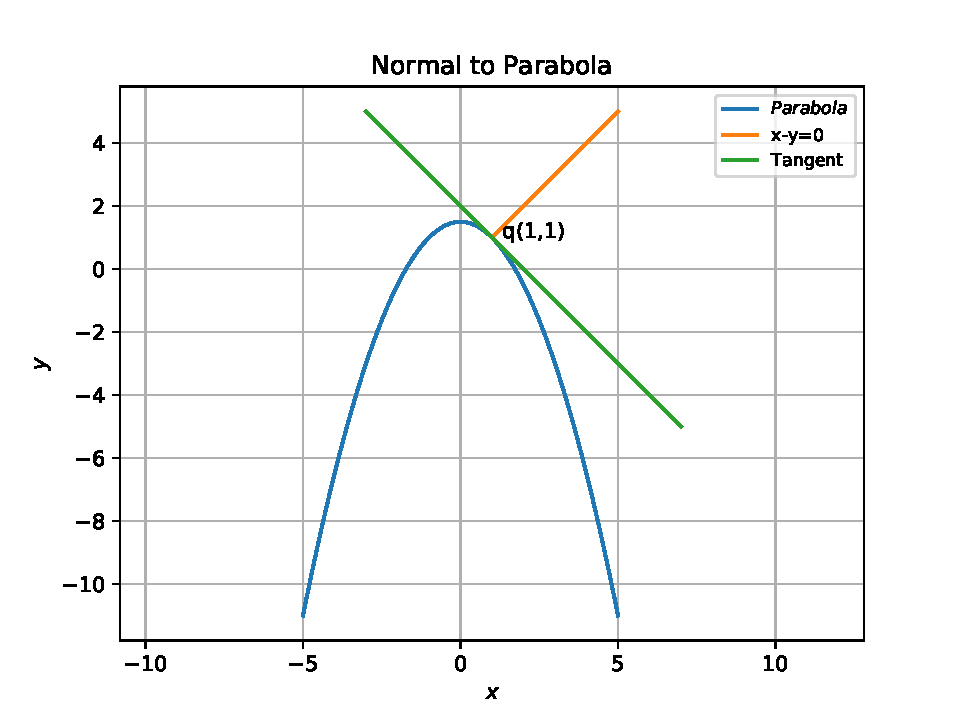
\includegraphics[width=\columnwidth]{figs/problem22.pdf}
	\end{center}
\caption{}
\label{fig:Fig1}
\end{figure}
\end{enumerate}
\end{document}
